\begin{figure*}[t]
    \centering
    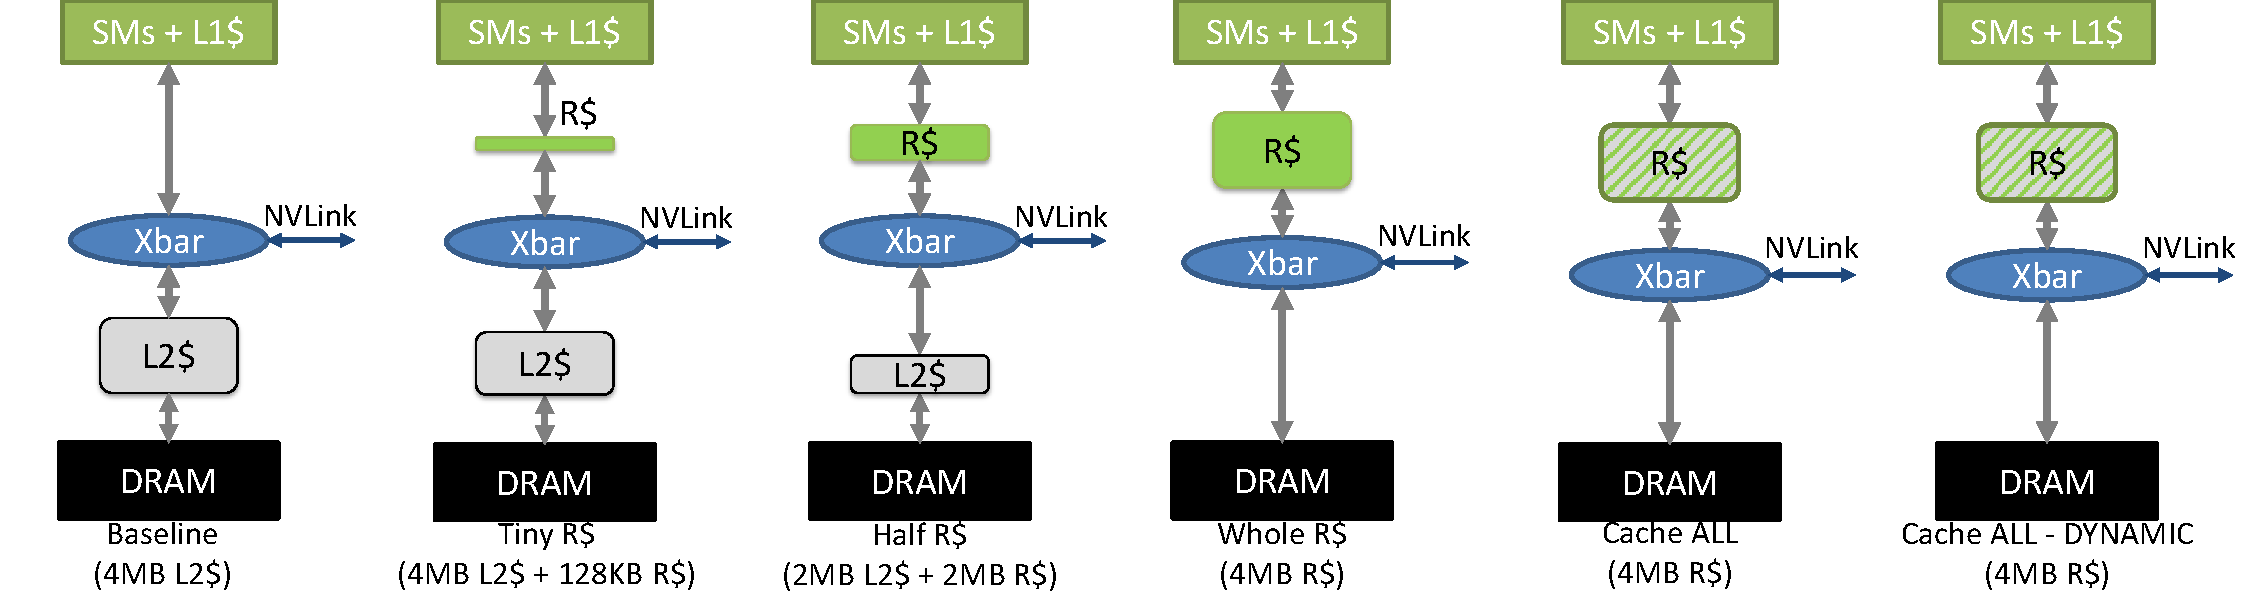
\includegraphics[width=1.0\textwidth]{figures/cache_configurations.pdf}
    \caption{Potential L2 cache organizations to balance capacity between NUMA remote
    local NUMA memory systems.}
    \label{fig:cacheorg}
\end{figure*}

\section{NUMA-Aware Cache Management}
\label{caching}
In Section~\ref{interconnect} we have shown that intersocket bandwidth is one
of the most important factors in achieving scalable NUMA-GPU performance. By
dynamically retraining the link to support asymmetric bandwidth configurations,
rather than a static 50--50 balance, we are able to improve the performance
of applications by XXX\%.  This improvement comes not from increasing the
absolute bandwidth of the link, but by using the existing link more efficiently.
Unfortunately, because either the outgoing or incoming links must be underutilized
for us to reallocate that bandwidth to the saturated link,  if both incoming and
outgoing links are saturated, this technique yields little improvement.
To improve performance in situations where dynamic link balancing is not effective,
system designers can increase link bandwidth, which is very expensive,
or try and decrease the amount of traffic that crosses the low bandwidth
communication channels.  To decrease off-chip memory traffic, architects typically
turn to caches to capture locality whenever possible.

GPU cache hierarchies differ from traditional CPU hierarchies where in they are
not supported by strong hardware coherence protocols~\cite{XXX}.  They also differ
from CPU protocols in that caches designed for a single uniform memory access GPU
may be both processor side (where some form of coherence is typically necessary)
or they may be memory side (where coherence is not necessary).  As described in
Table~\ref{methodology} and shown in Figure~\ref{fig:cacheorg}, a GPU today is
typically composed of relatively large SW managed coherent L1 caches that are 
physically proximal to the SM's, while a relatively small, distributed, non-coherent 
L2 cache resides memory side close to the memory controllers.  This
organization works well for GPUs because their SIMT processor designs often allow
for significant coalescing of requests to the same cache line, so having large
L1 caches reduces the need for global crossbar bandwidth.  By then placing the L2
caches memory-side, they do not need to participate in the coherence protocol (whatever
it may be).  Because of the fine grained interleaving of physical memory addresses
across memory channels, the L2 caches are inherently load balanced.

\subsection{Static Cache Partitioning}
In NUMA-designs interleaving memory references across the low bandwidth NUMA
interconnections results in poor performance, as shown in Figure~\ref{fig:motivation}.
Similarly, in NUMA-GPUs utilizing the traditional memory side L2 caches that 
depend on fine grained memory interleaving is a bad decision because these memory
side caches are not able to cache remote memory, and thus cannot reduce NUMA
interconnect traffic.  Arunkumar et. al have proposed that GPU L2 cache capacity
should be split between memory-side caches and a new processor-side L1.5 cache
that is an extension of the GPU L1 caches~\ref{Arunkumar2017} for caching remote
data only.  By balancing this capacity between local and remote caches they limit the 
need for invalidating the entire L2 cache capacity when extending the GPU coherence 
into the L1.5 cache while still minimizing crossbar bandwidth.  An example of this 
organization is shown in Figure~\ref{fig:cacheorg}.

In NUMA-GPUs the differential in local versus remote NUMA bandwidth is so great
that its not clear what the appropriate split between L1.5 and L2 capacity should
if using a similar organization.  To understand this trade-off Figure~\ref{fig:staticcache}
shows the performance improvement when moving from a local only (memory side cache)
to remote-only (processor side caching non-local data) cache.  Unlike the conclusions
of Arunkumar et. al, we find that for our multi-socket NUMA-GPU, allocating
100\% of the cache to remote data is by far the highest performing configuration.
The difference in this conclusion is likely due to the fact that their intra-GPU
crossbar has significantly more bandwidth than our multi-socket NUMA links, and thus
we need to dedicate more (all) of the GPU's L2 capacity to caching remote data, despite
the fact that SW based cache coherence will now effectively flush the entire L2 cache
on all GPUs when those operations occur.

\begin{figure}[t]
    \centering
    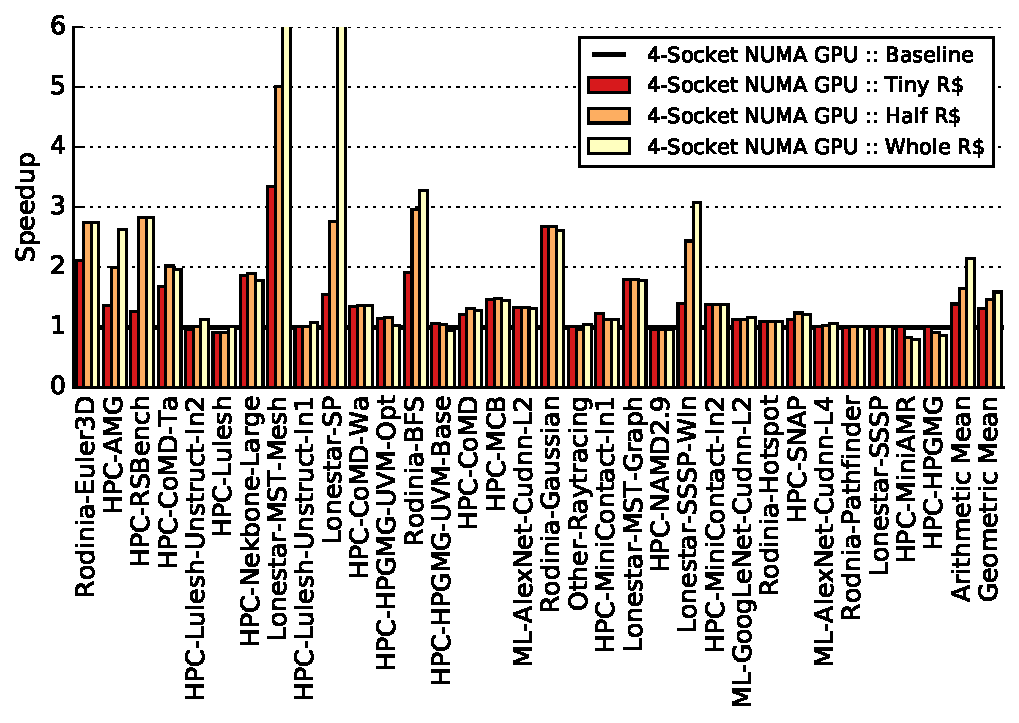
\includegraphics[width=1.0\columnwidth]{figures/plot_static_cache_WB.pdf}
    \caption{Performance comparison of static cache partitioning in a 4-socket GPU.}
    \label{fig:staticcaching}
\end{figure}

Static designs that allocate cache capacity to local memory, remote memory, or any
balance there of may achieve reasonable performance but they lack flexibility.  Much
like application phasing was shown to affect NUMA bandwidth needs, the ability to
dynamically partition cache capacity between local and remote memory has the potential
to improve performance under several situations.  First, when application phasing
results in some sockets within the NUMA-GPU to access data locally, while others
are accessing remote data, as shown in Figure~\ref{fig:link-motivation} dynamic
cache policy should outperform any static policy.  Second, while we show that many
applications will be able to completely utilize large NUMA-GPUs, this may not always
be the case.  GPUs within the data center are being virtualized and there is on-going
work to support concurrent execution of multiple kernels and/or processes within a
single GPU~\ref{}. If a large NUMA-GPU is subpartitioned, it is intuitive that system
software attempt to partition it along the NUMA boundaries so that a single small
application need not endure NUMA effects.  To effectively capture locality in such
a situation, NUMA-aware GPUs need to be able to flexibly move from 100\% local to
100\% remote caching at runtime, rather than be statically partitioned at design time.

\subsection{Dynamic Cache Partitioning}

Static L2 cache partitioning between local and remote data results in a GPU cache
organization in which the L1 caches contain both local and remote data but the GPU
L2 cache(s) will contain only local or remote data.  To-date, single socket GPUs
have not moved their memory-side caches to processor side because the overhead of
cache invalidation (due to coherence) is an unnecessary performance penalty, with
no performance upside to justify the cost.  However in a multi-socket NUMA GPU,
rather than statically partitioning the L2 cache at design time, the entire L2 cache
could be made an extension of the L1 and both local and remote data could dynamically
contend for capacity.  While conceptually simple, allowing both remote and local
memory accesses to contend for cache capacity in a NUMA system is flawed.

In non-NUMA systems, performance is maximized by optimizing for cache hitrate, which
minimizes off-chip memory system bandwidth.  In NUMA systems however, not all cache
misses have the same relative cost, and thus performance impact.  A cache miss to a 
NUMA-local memory address will have a smaller cost (in both terms of latency and bandwidth)
than a cache miss to a NUMA-remote memory address.  Thus, it should be beneficial
to dynamically skew cache allocation policy to preference caching of remote memory over local
data when it is determined the system is bottle necked on NUMA bandwidth.

We propose that rather than allowing both the L1 and L2 caches to be contended by local
and remote memory accesses,  both levels of the GPU cache hierarchy become NUMA-aware
and dynamically adjust their cache resources to preference caching of remote NUMA
data when it is determined that the NVLINK bandwidth in our hypothetical GPU is
oversubscribed.  We do this by implementing the following cache partitioning
algorithm:  \textbf{XXX UGI - at least another 2 paragraphs here on how we are actually doing this XXX}

\subsection{Results}

Figure~\ref{fig:dynamiccaching} shows the performance of a UMA cache policy versus
a NUMA-aware cache policy for our 4-socket GPU system.  By implementing our dynamic
policy, all caches in the multi-GPU system are able to independently change their local
behavior based on just four hardware counters monitoring the outgoing and incoming
NVLink bandwidth, utilizing the same sampling hardware and mechanism described in 
Section~\ref{interconnect}.  We see that dynamic partitioning can improve average GPU
performance by XXX\%.  More explain here.

\begin{figure}[t]
    \centering
    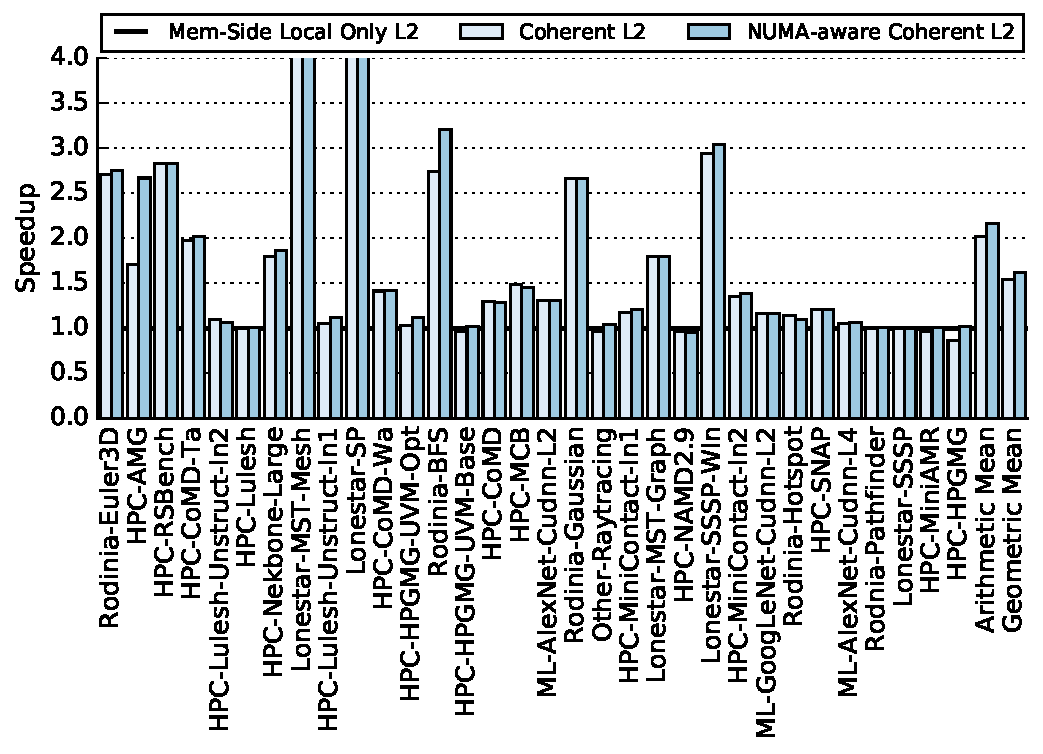
\includegraphics[width=1.0\columnwidth]{figures/plot_dynamic_cache_WB.pdf}
    \caption{Performance of NUMA-aware dynamic cache partitioning in a 4-socket GPU.}
    \label{fig:dynamiccaching}
\end{figure}

When extending the software controlled GPU coherence protocol into the GPU L2 caches,
L1 coherence operations (flushes) must also be extended into the GPU L2 caches.  To understand
the impact of these coherence operations on our dynamic cache performance we evaluated a hypothetical
cache implementation that need not flush on software defined boundaries.  This experiment
approximates a speed of light coherence implementation in which caches are still coherent but
there is no cost for maintaining that coherence.  In a 4-socket, 256 SM NUMA-GPU we observe
that the coherence overhead of current software based GPU coherence is only XXX\%.  We conclude
that despite some coherence overheads, the benefit of dynamic NUMA-aware coherent L2 caches
on multi-socket GPUs will be required to maximize both performance and GPU flexibility.

\begin{figure}[t]
    \centering
    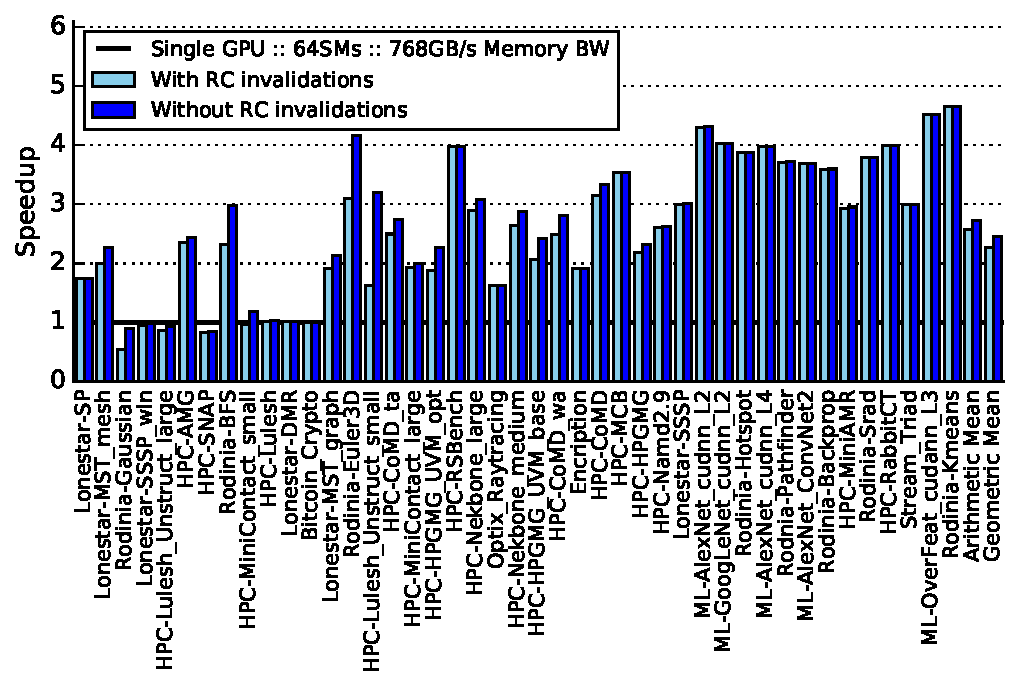
\includegraphics[width=1.0\columnwidth]{figures/plot_no_inval_WB.pdf}
    \caption{Performance overhead of extending current GPU software based coherence
    into the GPU L2 caches.}
    \label{fig:invalidations}
\end{figure}
